
My name is Keith Paulson and I am currently a first-year Ph.D. student in Computer Science.  My goals in the course are three-fold: improve my ability to express complex ideas in writing, study current state of art techniques in image generation, and start further developing my idea for dissertation.  I started at UCCS as a Masters Student in the Software Engineering Program.  I graduated last May.  

I have always been a reluctant writer, and prefer to present/perform tutorials.  I am active kinetic style learner.  I am hoping this course will help me mature my writing to be better able to express complicated ideas/concepts while maintaining my voice. As this learning style is not my preferred technique, it is more difficult for me to execute.  

I want to improve my understanding of the state of the art in particular in image generation/transformation through neural techniques like Generative Aggressive Networks (GANS).  I am also working to improve my math concepts as I find I have forgotten much of my undergraduate math.  I find this a challenge and distracting from the point of the paper.  However, at this stage it is necessary.

I plan to complete the Ph.D. program by Dec 2021, so I have a short time to build up my skills and complete my dissertation.  This seems aggressive to me, but I think it is important to set goals.  I plan to research image generation and transformation.  The current idea is to a combined GAN / geometric manipulation technique to allow the transformation of images.  I have taken Computer Vision, Computer Graphics, and my thesis and independent studies pursued the basics of machine learning tied to text processing.  I will be expanding this to images and vision over the next couple of years.

In short, I want to build up the basic and advanced skills needed to plan, develop, execute, and defend my dissertation in the next two years.  I know this is going to be a challenge, but hopefully, this course will help me get there.  

I also work full-time for MITRE Corporation. I am married to a wonderful woman and we share 2 incredible girls: ages 8 and 10.  We as a family have lived all over the country and world. We moved to Colorado Springs about 4 years ago.    My oldest girl was born in the Kingdom of Bahrain, and my youngest would have been born in Japan. In part due to the Triple Disaster (earthquake, tsunami, and Fukushima Daiichi nuclear plant), she was born in Florida, where we lived for a few years before moving here.  I enjoy meeting new people from different places and met a few fellow travelers  at a charity run as shown in Figure  \ref{fig:PaulsonLittleTall}.  Hint: I am in the middle.

\begin{figure}
	\centering
	\caption{Hanging out with some new friends and looking for some droids.}
	\label{fig:PaulsonLittleTall}
	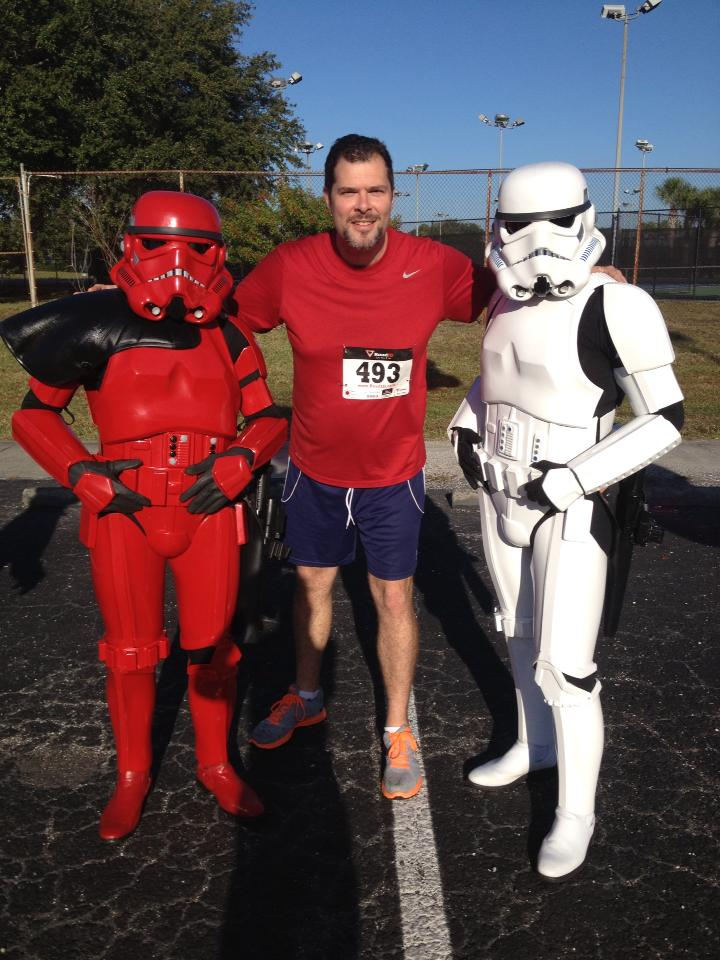
\includegraphics[width=0.7\linewidth]{PaulsonLittleTall}
\end{figure}

    \subsection{Questions and Answers}
    \subsubsection {Question \#1}
      This is where first question can be.   Please tell me your name and question.
    \subsubsection {Question \#2}
    This is where second question can be.  Please tell me your name and question.  
